This is a 1-D problem that consists of a domain with 2 regions of equal
saturation values $\frac{q}{\sigma}$, but with significantly individual values
of $\sigma$ and $q$ individually. The numerical solution should show no
evidence of the interface between the two regions.
Table \ref{tab:saturation} summarizes the test parameters.

%-------------------------------------------------------------------------------
\begin{table}[htb]\caption{Saturation Value Test Problem Summary}
\label{tab:saturation}
\centering
\begin{tabular}{l l}\toprule
\emph{Parameter} & \emph{Value}\\\midrule
Domain & $\mathcal{D} = (0,1)$\\
Initial Conditions & $u_0(\x)=0$\\
Boundary Conditions & $u(\x,t)=u_{inc}=1,\quad \x\in\partial\mathcal{D}^-,\quad t>0,$\\
   & $\partial\mathcal{D}^-=\{\x\in\partial\mathcal{D}:\mathbf{n}(\x)
     \cdot\mathbf{\Omega}<0\}$\\
Direction & $\mathbf{\Omega} = \mathbf{e}_x$\\
Cross Section & $\sigma(\x)=\left\{\begin{array}{c l}
   \sigma_0, & x\in[x_0,x_1]\\
   \sigma_1, & x\in(x_1,x_2]
   \end{array}\right.,\quad
   \left[\begin{array}{c}\sigma_0\\\sigma_1\end{array}\right] =
      \left[\begin{array}{c}1\\1\times 10^5\end{array}\right]$\\
   & $\left[\begin{array}{c}x_0\\x_1\\x_2\end{array}\right] =
      \left[\begin{array}{c}0\\0.5\\1\end{array}\right]$\\
Source & $q(\x,t)=\left\{\begin{array}{c l}
   q_0, & x\in[x_0,x_1]\\
   q_1, & x\in(x_1,x_2]
   \end{array}\right.,\quad
   \left[\begin{array}{c}q_0\\q_1\end{array}\right] =
      \left[\begin{array}{c}1\\1\times 10^5\end{array}\right]$\\
Speed & $c=1$\\
Exact Solution & $u(x,t) = 1$ \\
\bottomrule\end{tabular}
\end{table}
%-------------------------------------------------------------------------------

Figure \ref{fig:saturation} compares the solutions computed
for each scheme for this problem, and
Table \ref{tab:saturation_run_parameters} shows the run parameters used.
%-------------------------------------------------------------------------------
\begin{table}[ht]\caption{Saturation Value Test Problem Run Parameters}
\label{tab:saturation_run_parameters}
\centering
\begin{tabular}{l l}\toprule
\emph{Parameter} & \emph{Value}\\\midrule
Number of Cells & $N_{cell} = 2^5 = 32$\\
End Time & $t = 1$\\
CFL Number & $\nu = 0.5$\\
Time Integrator & SSPRK33\\\midrule
Entropy Function & $E(u) = \frac{1}{2}u^2$\\
Entropy Residual Coefficient & $c_E = 0.1$\\
Entropy Jump Coefficient & $c_J = 0.1$\\
Entropy Time Integrator & BE\\
\bottomrule\end{tabular}
\end{table}
%-------------------------------------------------------------------------------
\begin{figure}[ht]
   \centering
   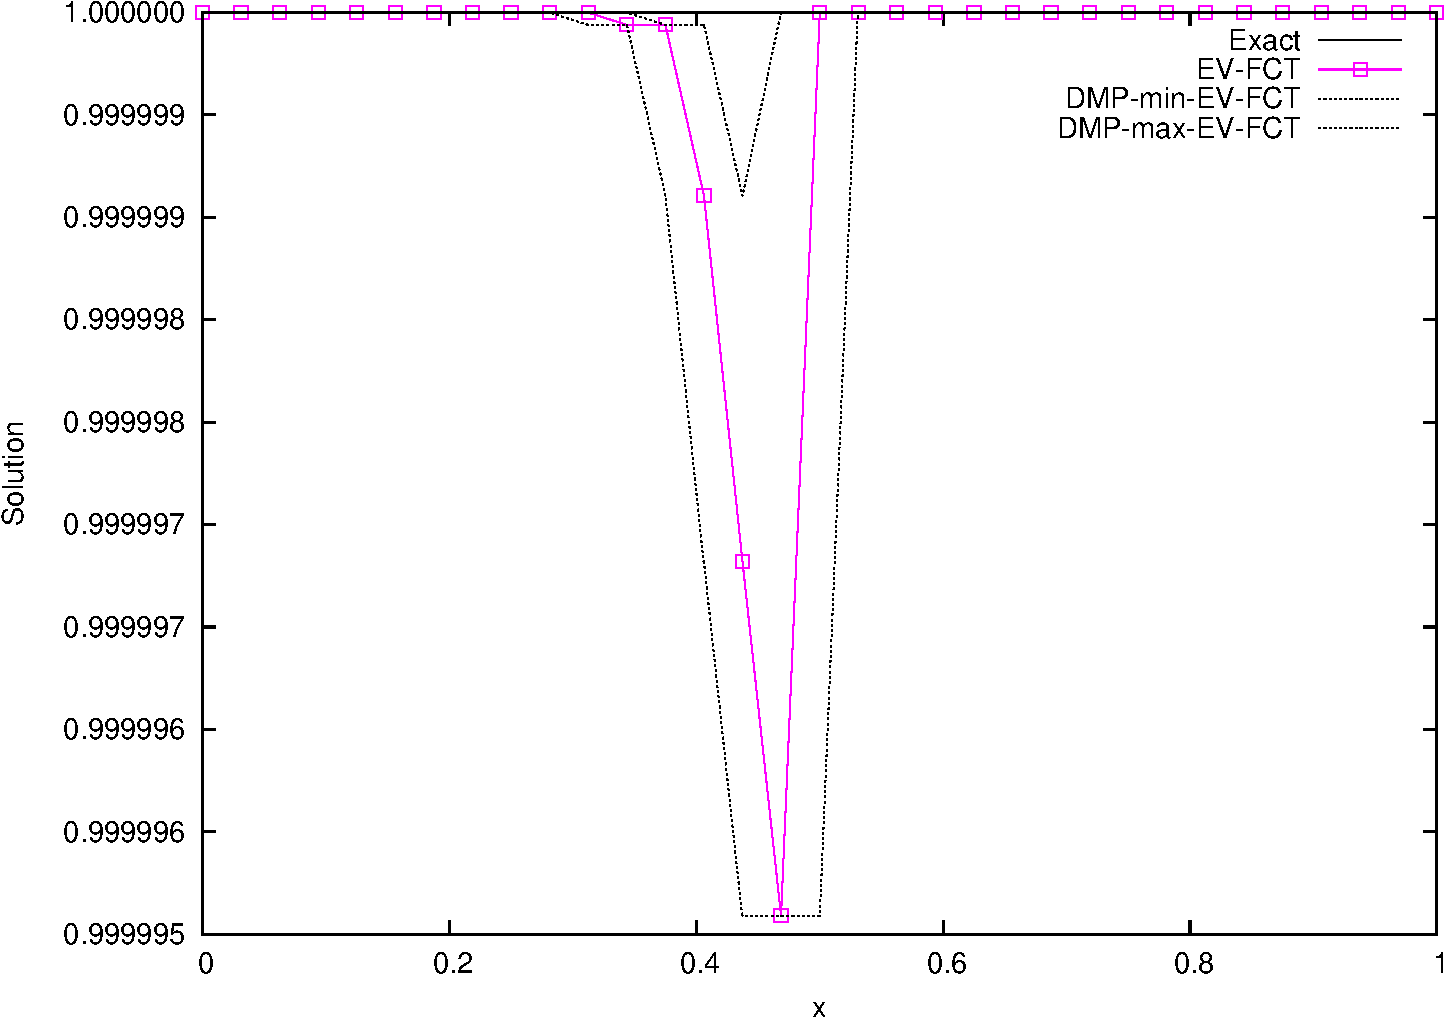
\includegraphics[width=0.9\textwidth]
     {\contentdir/results/transport/saturation/saturation.pdf}
   \caption{Comparison of Solutions for the Saturation Value Test Problem}
   \label{fig:saturation}
\end{figure}
%-------------------------------------------------------------------------------
